\documentclass{article}
\usepackage{graphicx}
\usepackage{subcaption}

\begin{document}
\begin{figure}
\centering

\begin{subfigure}[t]{.3\textwidth}
\centering
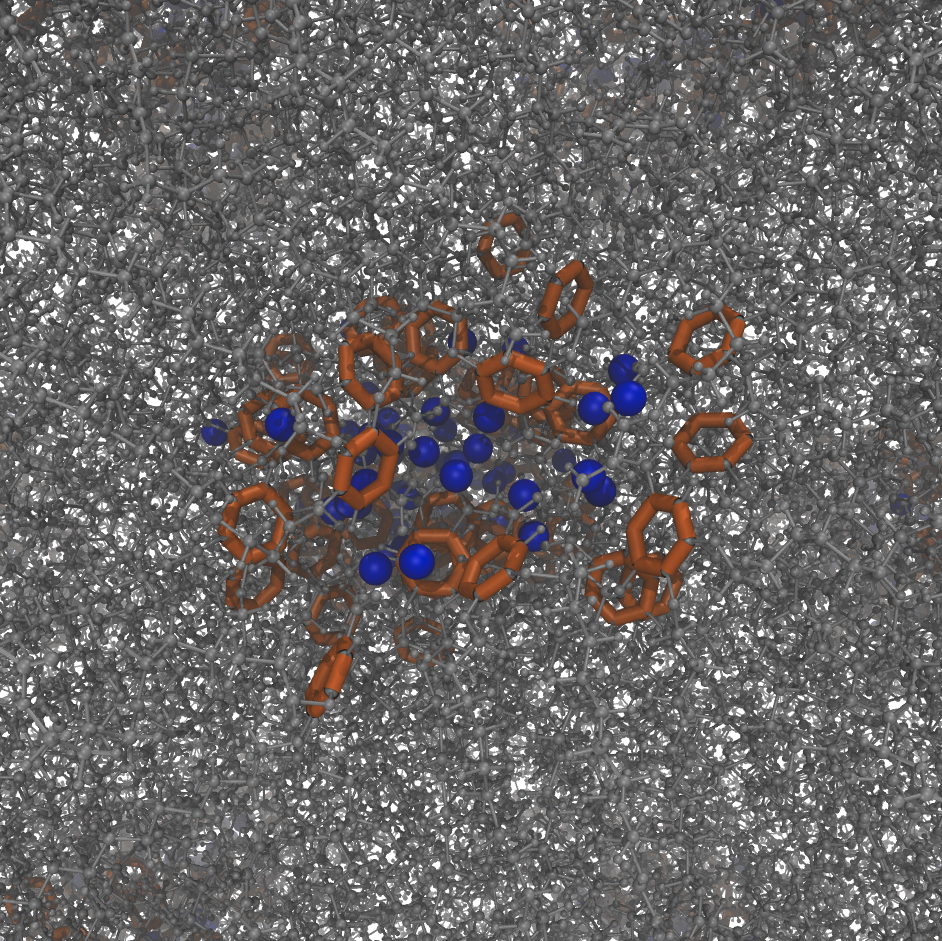
\includegraphics[width=\linewidth]{disordered_pore.png}
        \caption{}\label{fig:disordered_pore}
\end{subfigure}
%
\begin{minipage}[t]{.3\textwidth}
	test
\end{minipage}
%
\begin{subfigure}[t]{.3\textwidth}
\centering
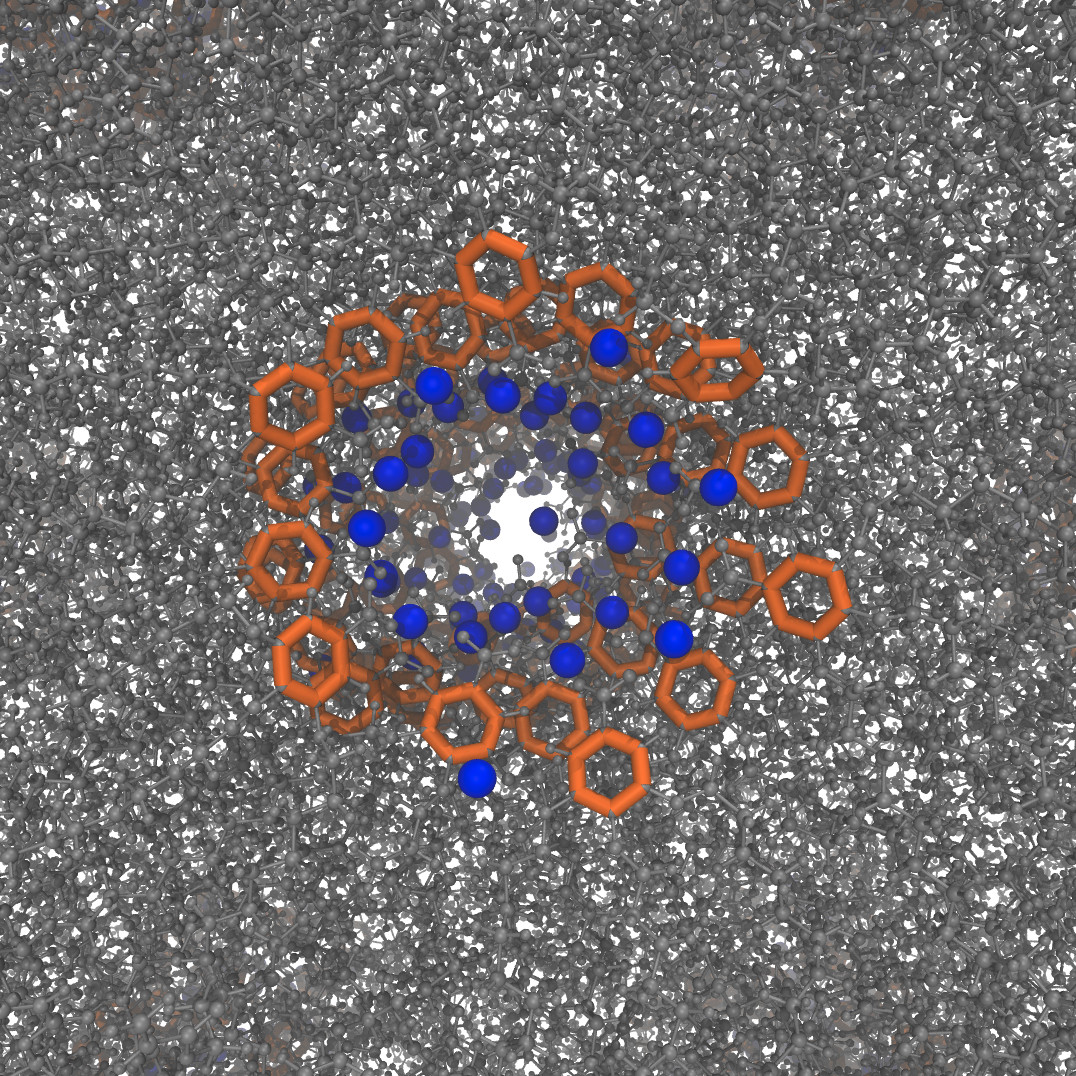
\includegraphics[width=\linewidth]{Ordered_Pore_orange.png}
\caption{}\label{fig:ordered_pore}
\end{subfigure}

\medskip

\begin{subfigure}[t]{.3\textwidth}
\centering
\vspace{0pt}% set the real top as the top
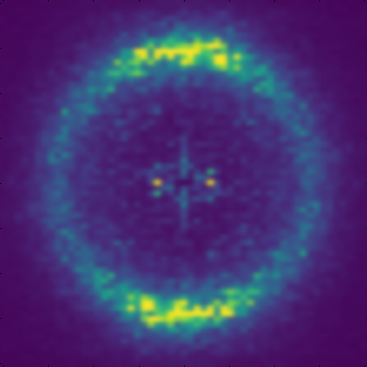
\includegraphics[width=\linewidth]{WAXS_disordered_pore_qyqz.png}
\caption{}\label{fig:disordered_XRD_sim}
\end{subfigure}
%
\begin{subfigure}[t]{.3\textwidth}
\centering
\vspace{0pt}% set the real top as the top
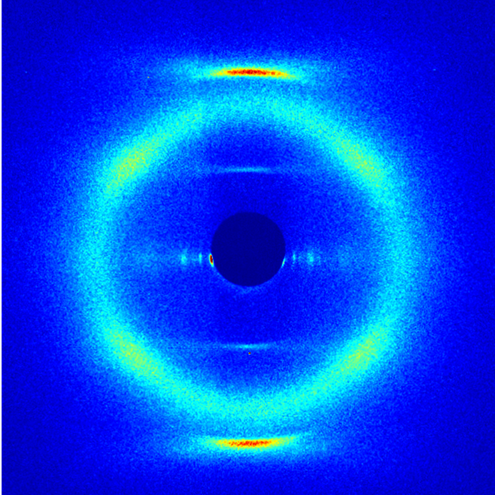
\includegraphics[width=\linewidth]{2DWAXS_experimental.png}
\caption{}\label{fig:experimental_XRD}
\end{subfigure}
%
\begin{subfigure}[t]{.3\textwidth}
\centering
\vspace{0pt}% set the real top as the top
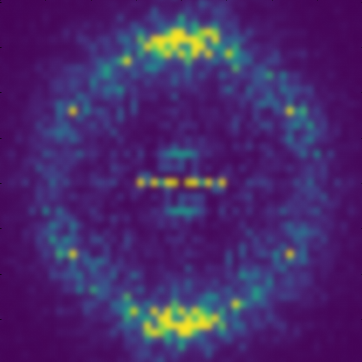
\includegraphics[width=\linewidth]{WAXS_ordered_pore_qyqz.png}
\caption{}\label{fig:Ordered_XRD_sim}
\end{subfigure}

\end{figure}

\end{document}
